
\section{How To Write A Composite Filter}

In general, most ITK filters implement one particular algorithm, whether it be
image filtering, an information metric, or a segmentation algorithm.  In the
previous section, we saw how to write new filters from scratch.  However, it is
often very useful to be able to make a new filter by combining two or more
existing filters, which can then be used as a building block in a complex
pipeline.  This approach follows the Composite pattern \cite{Gamma1995},
whereby the composite filter itself behaves just as a regular filter, providing
its own (potentially higher level) interface and using other filters (whose
detail is hidden to users of the class) for the implementation.  This composite
structure is shown in Figure~\ref{fig:CompositeFilterStages}, where the various
\code{Stage-n} filters are combined into one by the \code{Composite} filter.
The \code{Source} and \code{Sink} filters only see the interface published by
the \code{Composite}.  Using the Composite pattern, a composite filter can
encapsulate a pipeline of arbitrary complexity.  These can in turn be nested
inside other pipelines.

\begin{figure}
  \centering
  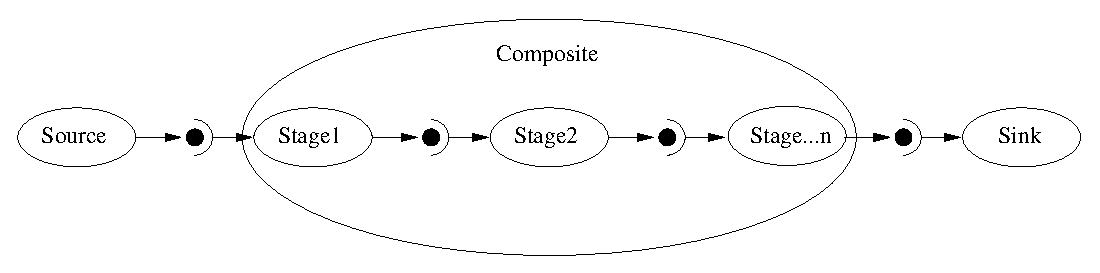
\includegraphics[width=0.9\textwidth]{CompositeFilterStages.eps}
  \itkcaption[Composite Filter Concept]{A Composite filter encapsulates a number of other filters.} 
  \label{fig:CompositeFilterStages}
\end{figure}

\subsection{Implementing a Composite Filter}

There are a few considerations to take into account when implementing a
composite filter.  All the usual requirements for filters apply (as
discussed above), but the following guidelines should be considered:

\begin{enumerate}

\item The template arguments it takes must be sufficient to instantiate all of
the component filters.  Each component filter needs a type supplied by either
the implementor or the enclosing class.  For example, an
\code{ImageToImageFilter} normally takes an input and output image type (which
may be the same).  But if the output of the composite filter is a classified
image, we need to either decide on the output type inside the composite filter,
or restrict the choices of the user when she/he instantiates the filter.

\item The types of the component filters should be declared in the header,
  preferably with \code{protected} visibility.  This is because the
  internal structure normally should not be visible to users of the class,
  but should be to descendent classes that may need to modify or customize
  the behavior. 

\item The component filters should be private data members of the composite
  class, as in \code{FilterType::Pointer}. 

\item The default constructor should build the pipeline by creating the
  stages and connect them together, along with any default parameter
  settings, as appropriate. 

\item The input and output of the composite filter need to be grafted on to
  the head and tail (respectively) of the component filters. 

\end{enumerate}

This grafting process is illustrated in Figure~\ref{fig:CompositeExamplePipeline}. 


\subsection{A Simple Example}

\begin{figure}
  \centering
  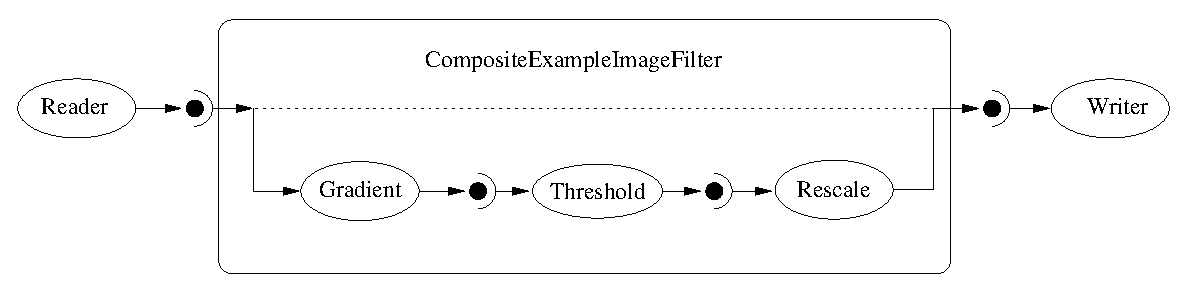
\includegraphics[width=0.9\textwidth]{CompositeExamplePipeline.eps}
  \itkcaption[Composite Filter Example]{Example of a typical composite filter. Note that the output of the last filter in the internal pipeline must be grafted into the output of the composite filter.} 
  \label{fig:CompositeExamplePipeline}
\end{figure}

\input{CompositeFilterExample.tex}

%---------------------------------------------------------------------------
